\documentclass[12pt,a4paper]{article}
\usepackage[utf8]{inputenc}
\usepackage[utf8]{vietnam}
\usepackage{amsmath}
\usepackage{amsfonts}
\usepackage{amssymb}
\usepackage{indentfirst}
\usepackage{graphicx}
\usepackage{subfig}
\usepackage{enumerate}
\usepackage[left=2cm,right=2cm,top=2cm,bottom=2cm]{geometry}
\graphicspath{{images/}}
\everymath{\displaystyle}

\title{\textbf{Bài tập Điều khiển quá trình \bigskip \\ Chủ đề Mô hình hóa lý thuyết}}
\author{Sưu tầm: Thi Minh Nhựt \and Email: thiminhnhut@gmail.com}
\date{Thời gian: \today}

\begin{document}
    \maketitle
    \section{Bài tập 1}
        \paragraph{Giả thiết}
        Cho hệ thống như hình \ref{baitap1}: Bình chứa thứ nhất có tiết diện là $A_1$ và bình chứa thứ hai có tiết diện là $A_2$. Các lưu lượng ra $Q_b$ và $Q_c$ được xác định như sau: $Q_b = C_{db}a_b\sqrt{2g(H_1 - H_2)}$ và $Q_c = C_{dc}a_c\sqrt{2gH_2}$
            \begin{figure}[htp]
                \begin{center}
                    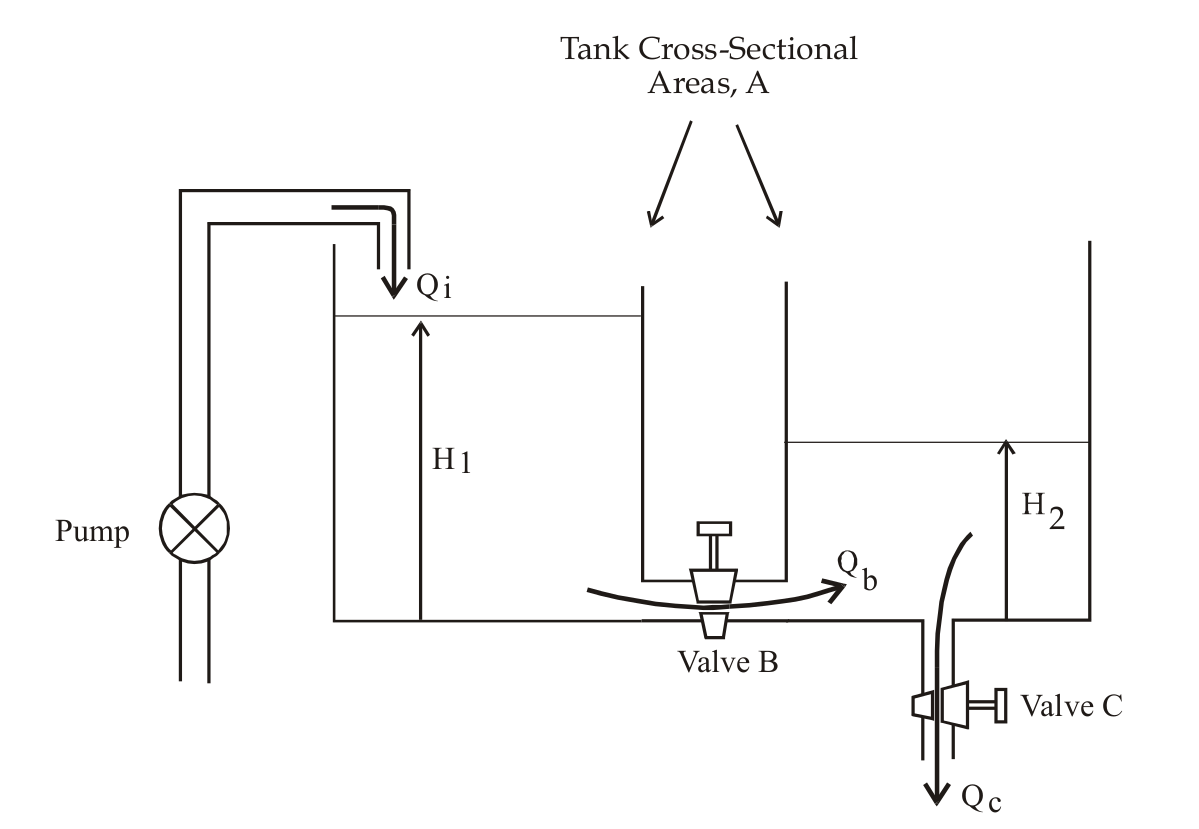
\includegraphics[scale=.3]{bai1}
                \end{center}
                \caption{Hệ thống 2 bình chứa} \label{baitap1}
            \end{figure}

        \paragraph{Yêu cầu}
            \begin{enumerate}[a.]
                \item Xác định các biến vào, biến ra, biến điều khiển, biến cần điều khiển và biến nhiễu.
                \item Viết phương trình mô tả quan hệ giữa các biến.
                \item Tuyến tính hóa mô hình tại điểm làm việc cân bằng.
                \item Tìm hàm truyền $G(s) = \dfrac{H_2(s)}{Q_i(s)}$                                    
            \end{enumerate}
         
\section{Bài tập 2}
        \paragraph{Giả thiết}
        Cho hệ thống như hình \ref{baitap2}:  Các lưu lượng ra $q_1$ và $q_0$ được xác định như sau: $q_1 = \dfrac{h_1 - h_2}{R_1}$ và $q_0 = \dfrac{h_2}{R_2}$
            \begin{figure}[htp]
                \begin{center}
                    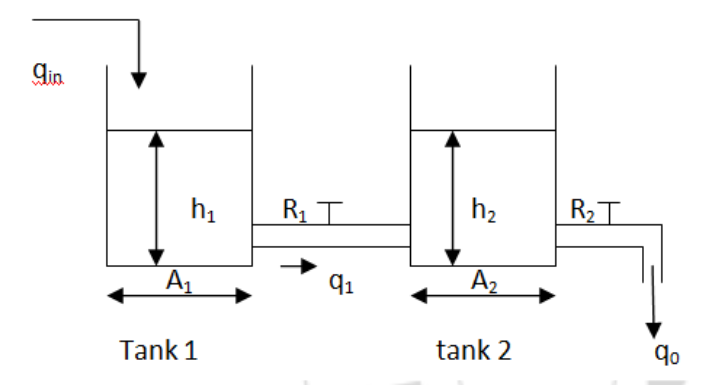
\includegraphics[scale=.5]{bai2}
                \end{center}
                \caption{Hệ thống 2 bình chứa} \label{baitap2}
            \end{figure}

        \paragraph{Yêu cầu}
            \begin{enumerate}[a.]
                \item Xác định các biến vào, biến ra, biến điều khiển, biến cần điều khiển và biến nhiễu.
                \item Viết phương trình mô tả quan hệ giữa các biến.
                \item Tuyến tính hóa mô hình tại điểm làm việc cân bằng.
                \item Tìm hàm truyền $G(s) = \dfrac{H_2(s)}{Q_{in}(s)}$                                    
            \end{enumerate}
\end{document}